\subsection{Playlist}
This subsystem will contain all the information on a users playlists and display it to them.

\begin{figure}[h!]
	\centering
 	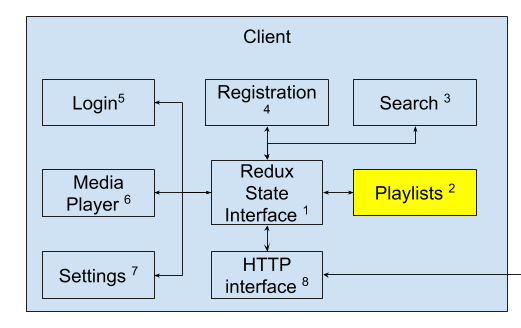
\includegraphics[width=0.60\textwidth]{images/client/client_playlists.png}
 	\caption{Playlist subsystem}
\end{figure}

\subsubsection{Subsystem Hardware}
No hardware is used for this layer. The playlist component will be a component of the home page which will be hosted on Heroku.

\subsubsection{Subsystem Operating System}
No OS is required in order for the playlist component to work properly.

\subsubsection{Subsystem Software Dependencies}
We will be using React.js 16.8.0-alpha.1 for our framework and will be using the Fetch API from Mozilla.

\subsubsection{Subsystem Programming Languages}
We will be using JavaScript ES6

\subsubsection{Subsystem Data Structures}
The data structure of the playlist is going to be an object that contains a playlist name as the key with its value being an object of song names and artists. This structure may change depending on what various music services API returns.

\subsubsection{Subsystem Data Processing}
When a use chooses a playlist that they would like to view, the Front End will take that choice in order to display the proper playlist by comparing it to the stored music data.

\newpage